
\section{Pull-back Prior}\label{sec:pull_back_prior}

\subsection{Intuition of Pull-back Prior}\label{subsec:intuition}

The formula of Pull-back Prior is given by:
\begin{equation}\label{eq:pull_back_prior}
	p_\lambda(z) = \frac{1}{Z} p_\mathcal{N}(z) \cdot e^{- \beta D(G(z))} \tag{4}
\end{equation}
where $p_\mathcal{N}$ is a simple prior, $D$ is a discriminator, $G$ is a generator, $f_\lambda(z)$ denotes $p_\mathcal{N}(z) e^{- \beta D(G(z))}$, $Z$ is the partition function $Z = \int_{\mathcal{Z}} f_\lambda(z) \dd z$ and $\beta$ is a learnable scalar.

A design proposition of Pull-back Prior is that we increase $p_\lambda(z)$ where $z$ generates better data and decrease $p_\lambda(z)$ where $z$ generates worse data. In Pull-back Prior, 
$D$ is a discriminator to assess the quality of $x$, where smaller $D(x)$ indicates $x$ being more similar to real data, as shown in \cref{fig:interpolate}. Such discriminator $D(x)$ is defined on $x$, and the pull-back discriminator on $z$ is defined by $D(G(z))$, where $D(G(z))$ represents the ability of $z$ that can generate data with high quality. To increase $p_\lambda(z)$ at the better $z$ and decrease $p_\lambda(z)$ at the worse $z$, we modify $p_\mathcal{N}(z)$ by $\beta D(G(z))$, and then normalize it by $Z$. Finally, we obtain the basic formula of Pull-back Prior. 

The theoretical derivation for Pull-back Prior is provided in \cref{subsec:inference}. However, it remains questions about how to obtain $D$ and $G$, determine $\beta$, and calculate $Z$. 

\begin{figure}[tb]
	\centering
	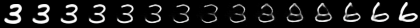
\includegraphics[width=0.9\columnwidth]{../figures/interpolate}
	\caption{
	The discriminators on above images (generated by linear interpolation of two sample from $q_\phi(z)$), are better at both sides and worse at the middle, which validates the intuition that a discriminator can assess the quality of images. Moreover, the density of $z$ which generates better images will increase, and the density of $z$ which generates worse images will decrease. 
%2825-plot_samples mean and std is 9.528099, 0.0050279954
%[array([[9.547822]], dtype=float32), array([[9.583102]], dtype=float32), array([[9.603901]], dtype=float32), array([[9.626318]], dtype=float32), array([[9.633714]], dtype=float32), array([[9.632847]], dtype=float32), array([[9.631333]], dtype=float32), array([[9.640044]], dtype=float32), array([[9.631817]], dtype=float32), array([[9.654361]], dtype=float32), array([[9.641564]], dtype=float32), array([[9.600273]], dtype=float32), array([[9.559095]], dtype=float32), array([[9.533435]], dtype=float32), array([[9.468535]], dtype=float32)]
%Normalized is [  3.92263684,  10.93934971,  15.07598834,  19.53442519,
%        21.00538915,  20.83295462,  20.53184058,  22.26434018,
%        20.62810161,  25.11179704,  22.56664754,  14.35442841,
%         6.16468344,   1.06125793, -11.84647066]
	}
	\label{fig:interpolate}
\end{figure}

\subsection{How to obtain $D$ and $G$}\label{subsec:determine_D_and_G}
We choose $G(z) = \E_{p_\theta(x|z)} x$ in our model, \IE the mean of the $p_\theta(x|z)$. Notice that $p_\theta(x|z)$ is chosen to be a Discretized Logistic~\protect\cite{salimans2017pixelcnn++} or a Bernouli in our experiments. $G(z)$ is generated by a neural network and it is set as the mean of $p_\theta(x|z)$. 

$D$ plays an important role in Pull-back Prior. We shall propose two ways to obtain $D$ in \cref{subsec:naive_vaepp} and \cref{subsec:improve_of_vaepp}, and compare them later in our experiments. 

\subsection{How to determine $\beta$}\label{subsec:determine_beta}

Theoretically, $\beta$ in \cref{eq:pull_back_prior} represents how far $p_\lambda$ is from $p_\mathcal{N}$, as proved in \cref{subsec:inference}.
%but how to decide the value of $\beta$? When $\beta$ is smaller, the difference between $p_\lambda$ and $p_\mathcal{N}$ is less, \IE the influence of discriminator is severely limited. When $\beta$ is larger, $p_\lambda$ is farther from $p_\mathcal{N}$. Noticing that in \cref{eq:final_optimization}, we simplify the optimization of $D$ by an approximated $D$, if $p_\lambda$ is too far from $p_\mathcal{N}$, this approximation will become invalid. 
%Consequently, $\beta$ should be set to an appropriate value which can't severely limit the influence of discriminator and could ensure that approximated $D$ is valid. 
%It is important to realize that the Pull-back Prior is serving for better ELBO. 
%Whatever the function family of $p_\lambda$ is limited or approximation $D$ is invalid, the ELBO will suffer. 
%Therefore, it is reasonable to search $\beta$ by the optimization for ELBO ($\lambda$ contains $\beta$ and $\omega$, which is the parameters of $D$):
To maximize ELBO, we can obtain the optimal $\beta$ by:
\begin{equation}
	\beta = \arg \min_{\beta} \mathcal{L}(\theta, \phi, \lambda) = \arg \min_{\beta} \mathcal{L}(\theta, \phi, \beta, \omega) \tag{5}
\end{equation}
The gradient $\partial \mathcal{L}/\partial \beta$ is:
\begin{align*}\label{eq:behavior_of_beta}
\frac{\partial \ln Z}{\partial \beta} &= \frac{1}{Z} \int_{\mathcal{Z}} p_\mathcal{N}(z) e^{-\beta D(G(z))} \cdot (-D(G(z))) \dd z \\
&=  \E_{p_\lambda(z)} [- D(G(z))]  \\
\frac{\partial \mathcal{L}}{\partial \beta} &= \E_{q_\phi(z)}[ -D(G(z))] - \frac{\partial \ln Z}{\partial \beta} \\
&= - \E_{q_\phi(z)}[ D(G(z))] + \E_{p_\lambda(z)}[ D(G(z))]   \tag{6}
\end{align*}
The 1st term in \cref{eq:behavior_of_beta} is the mean of the discriminator on reconstructed data (reconstructed data are nearly same as real data in VAE, after only few epochs in training). 
The 2nd term in \cref{eq:behavior_of_beta} is the mean of the discriminator on data generated from $p_\lambda$. 
Hence, $\partial \mathcal{L}/\partial \beta = 0$ means that the discriminator can't distinguish reconstructed data and generated data when the training converges. It coincides with the philosophy of GANs that the discriminator can't distinguish the real data and generated data when the generator is well-trained.	

Noticing that $p_\mathcal{N}$ is a special case of $p_\lambda$ where $\beta = 0$, Pull-back Prior is indeed a general form of the standard Gaussian.  We shall compare their performance in experiments. 

\subsection{The upper-bound of $Z$}\label{subsec:determine_z}

It is difficult to calculate the exact partition function $Z$. Fortunately for VAE, it is acceptable to obtain an upper-bound of $Z$, denoted by $\hat{Z}$. Using the upper-bound $\hat{Z}$ in training and evaluation, we can obtain lower-bounds of log-likelihood and ELBO (note, $\hat{p}_\theta(x) \leq p_\theta(x)$ indicates $\ln \hat{p}_\theta(x) \leq \ln p_\theta(x)$):
\begin{align*}
	\hat{p}_\theta(x) = \int \frac{p_\theta(x|z) f_\lambda(z)}{\hat{Z}}  \dd z &\leq \int \frac{p_\theta(x|z) f_\lambda(z)}{Z} \dd z = p_\theta(x)  \\
	\mathcal{\hat{K}} = \E_{q_\phi(z)} \ln \frac{1}{\hat{Z}} f_\lambda(z) &\leq \E_{q_\phi(z)} \ln \frac{1}{Z}  f_\lambda(z) = \mathcal{K}   \\
    \mathcal{\hat{L}} =  \mathcal{I} + \mathcal{J} + \mathcal{\hat{K}} &\leq \mathcal{I} + \mathcal{J} + \mathcal{K} = \mathcal{L}
\end{align*}

The upper-bound $\hat{Z}$ in our model is derived as follows:
\begin{align*}\label{eq:Z_estimator}
    \hat{Z} = \E_{p^*(x)}\E_{q_\phi(z|x)} \frac{f_\lambda(z)}{\frac{1}{N}q_\phi(z|x)} \geq
	\E_{q_\phi(z)}\frac{f_\lambda(z)}{q_\phi(z)} = Z \tag{7}
\end{align*}
The fact that $\hat{Z}$ is an upper-bound of $Z$ comes from:
\begin{equation*}
	\frac{q_\phi(z|x)}{N} \leq \frac{1}{N}\sum_{i=1}^N q_\phi(z|x^{(i)}) \approx \E_{p^*(x)}q_\phi(z|x) = q_\phi(z)
\end{equation*}
%The key of \cref{eq:Z_estimator} is the choice of $\hat{q}_\phi(z|x)$. For any given $z$, although it is intractable to compute the exact density of $q_\phi(z)$, it is feasible to compute $\hat{q}_\phi(z|x)$, which is a lower-bound of $q_\phi(z)$ for any $x$ sampled from $p^*(x)$:

% where $x^{(j)}$ is any sample in dataste and $N$ is the size of training set. $x^{(j)}$ plays an important role here. %If $z$ must be sampled from a real data $x^{(k)}$, $x^{(j)}$ is chosen as the $x^{(k)}$. 
%To reduce the gap between $\hat{q}_\phi(z)$ and $q_\phi(z)$, $q_\phi(z|x^{(j)})$ should be one of the largest in the summation. Therefore, we firstly sample $x^{(j)}$ form dataset, and then sample $z$ from $q_\phi(z|x^{(j)})$. By this way, $q_\phi(z|x^{(j)})$ is large enough. 
%
%In MNIST and other Bernouli image datasets, the number of Bernouli images might be numerous and $\hat{q}_\phi(z)$ might be underestimiated due to the large $N$. 
%Since the size of real images $M$, is much smaller than the size of Bernouli images $N$, we use $q_\phi(z|e)$ instead of $q_\phi(z|x)$ to estimate $\hat{q}_\phi(z)$, where $e$ means the real image and $x$ means the Bernouli image. 
%Formally, $p^*(e)$ denotes the distribution of real images and $p^*(x|e)$ denotes the Bernouli sampling process from $e$. Notice $q_\phi(z|e) = \E_{p^*(x|e)} q_\phi(z|x)$ and $q_\phi(z) = \E_{p^*(x)} q_\phi(z|x) = \E_{p^*(e)} q_\phi(z|e)$. 
%Having $q_\phi(z|e)$, we could easily obtain $\hat{Z}$ by 
%\begin{align*}~\label{eq:another_Z_estimator}
%	\hat{Z} &= \E_{p^*(e)} \E_{q_\phi(z|e)} \frac{f_\lambda(z)}{\hat{q}_\phi(z|e)} \geq \E_{q_\phi(z)} \frac{f_\lambda(z)}{q_\phi(z)} = Z \\
%	\hat{q}_\phi(z|e) &= \frac{q_\phi(z|e)}{M} = \frac{1}{M}\sum_{i=1}^M q_\phi(z|e^{(i)}) \leq q_\phi(z) \tag{8}
%\end{align*}  
%
%We propose ELBO to train a VAE based on $q_\phi(z|e)$:
%\begin{align*}~\label{eq:another_elbo}
%	&\E_{p^*(x)} \ln p_\theta(x) = \E_{p^*(e)} \E_{p^*(x|e)} \ln \E_{q_\phi(z|e)} \frac{p_\theta(x|z)p_\lambda(z)}{q_\phi(z|e)} \\
%	 &\geq \E_{p^*(e)} \E_{p^*(x|e)} \E_{q_\phi(z|e)} \ln \frac{p_\theta(x|z)p_\lambda(z)}{q_\phi(z|e)} \tag{9} %\\
%	 %&= \E_{p^*(x)} \ln p^*(x) - \E_{p^*(e)} \E_{p^*(x|e)} KL(q_\phi(z|e), p_\theta(z|x))
%\end{align*} 
%\cref{eq:another_elbo} is similar to the original ELBO, and the conclusions in this paper hold for \cref{eq:another_elbo} by repeating derivations for \cref{eq:another_elbo}. $\mathcal{L}(\theta, \phi, \lambda)$ denotes \cref{eq:another_elbo} in Bernouli image datasets.  %Moreover, the situation without Bernouli images is a special case where $p^*(x|e) = \delta(x - e)$. % Additionally, when $p_\theta(x|z)$ and $p^*(x|e)$ is both Bernouli, term $\E_{p^*(x|e)} \ln p_\theta(x|z)$ has analytical solution $x\log e+(1-x)\log(1-e)$, which could make the training and evaluation more stable (don't need sample $x$). 
%In the dataset without Bernouli image, $e, x$ both means real image, and $p^*(x|e) = \delta(x - e)$ where $\delta$ is Dirac delta function. 

In previous VAE literatures and our paper, it is a common practice to dynamically sample 0/1 binary images (which is exactly the $x$ of our VAE and may other paper's) from real-value grayscale images (whose distribution is denoted by $p^*(e)$). Each pixel value of $e$ is normalized to $[0, 1]$, and is used as the probability of the corresponding pixel of $x$ being 1 (denoted by $p^*(x|e)$). In such situation, even when the size $M$ of original grayscale image dataset is moderate, the size $N$ of the sampled images dataset is exponentially large. Hence, we shall severely underestimate $q_\phi(z)$ if directly using \cref{eq:Z_estimator}. Because of this, we consider to use $p^*(e)$ instead of $p^*(x)$ to estimate $q_\phi(z)$ in such datasets (called Bernouli datasets in our paper). Given that $p^*(x) = \E_{p^*(e)} p^*(x|e)$, we shall have:
\begin{align*}~\label{eq:another_q_z}
	q_\phi(z) = \E_{p^*(e)} \E_{p^*(x|e)} q_\phi(z|x) = \E_{p^*(e)}q_\phi(z|e) \tag{8}
\end{align*}
where $q_\phi(z|e)$ denotes $\E_{p^*(x|e)} q_\phi(z|x)$. \cref{eq:another_q_z} suggests that we may train a variational encoder $q_\phi(z|e)$ instead of $q_\phi(z|x)$ along with a generative decoder $p_\theta(x|z)$, while the log-likelihood estimator is still correct:
\begin{align*}
	\E_{p^*(x)} \log p_\theta(x) &= \E_{p^*(e)} \E_{p^*(x|e)} \log p_\theta(x) \\
	&= \E_{p^*(e)} \E_{p^*(x|e)} \log \E_{q_\phi(z|e)} \frac{p_\theta(x, z)}{q_\phi(z|e)}
\end{align*}
Based on this idea, we then derive $\hat{Z}$ and ELBO as:
\begin{align*}~\label{eq:another_elbo}
    &\hat{Z} = \E_{p^*(e)}\E_{q_\phi(z|e)} \frac{f_\lambda(z)}{\frac{1}{M}q_\phi(z|e)} \geq
	\E_{q_\phi(z)}\frac{f_\lambda(z)}{q_\phi(z)} = Z \\
	&\E_{p^*(x)} \ln p_\theta(x) = \E_{p^*(e)} \E_{p^*(x|e)} \ln \E_{q_\phi(z|e)} \frac{p_\theta(x|z)p_\lambda(z)}{q_\phi(z|e)} \\
    &\geq \E_{p^*(e)} \E_{p^*(x|e)} \E_{q_\phi(z|e)} \ln \frac{p_\theta(x|z)p_\lambda(z)}{q_\phi(z|e)} \tag{9} \\
    &= \E_{p^*(x)} \ln p^*(x) - \E_{p^*(e)} \E_{p^*(x|e)} KL(q_\phi(z|e), p_\theta(z|x)) 
\end{align*}
\cref{eq:another_elbo} is similar to the original ELBO, and the conclusions in this paper hold for \cref{eq:another_elbo} by repeating derivations for \cref{eq:another_elbo}. $\mathcal{L}(\theta, \phi, \lambda)$ denotes \cref{eq:another_elbo} in Bernouli datasets. 
For other datasets, the distribution $p^*(e)$ and $p^*(x)$ is same, and we shall use $p^*(x|e) = \delta(x - e)$, where $\delta$ is Dirac delta function.%, for convenience of algorithm descriptoin.  

Review the estimation of $Z$. By the theory of importance sampling, $p_\lambda$ is the optimal choice for the proposal distribution in the estimation of $Z$. However, it is intractable to sample from $p_\lambda$. 
\cite{bauer2019resampled} uses $p_\mathcal{N}$ as the proposal distribution to estimate $Z$ but when $KL(p_\mathcal{N}, p_\lambda)$ is high, the variance of this estimation will be large. 

In our experiments, $KL(q_\phi, p_\lambda)$ is much smaller than $KL(p_\mathcal{N}, p_\lambda)$. Therefore, we choose $q_\phi(z)$ as the proposal distribution and replace $q_\phi(z)$ by $\hat{q}_\phi(z|x)$, to obtain the lower-bound of $\hat{Z}$ in \cref{eq:Z_estimator}. The variance of $\hat{Z}$ is acceptable in experiments.  
In training, $p_\mathcal{N}(z)$ could be used together with $q_\phi(z)$, as the proposal distributions, since $KL(p_\mathcal{N}, p_\lambda)$ is small in the beginning of training.
 